\documentclass{article}

\usepackage{aligned-overset}
\usepackage{amsmath}
\usepackage{amssymb}
\usepackage{bbm}
\usepackage[shortlabels]{enumitem}
\usepackage{genealogytree}
\usepackage{hyperref}
\usepackage[utf8]{inputenc}
\usepackage{interval}
\intervalconfig{
  soft open fences
}
\usepackage{mathtools}
\usepackage{pgfplots}
\usepackage{physics}
\usepackage{tikz}
\usetikzlibrary{positioning}
\usepackage{xcolor}
\definecolor{light-gray}{gray}{.9}

\author{Karsten Lehmann}
\date{09.11.2020}
\title{Hausaufgabe 02 Analysis - Grundlegende Konzepte}

\begin{document}


\maketitle
\newpage

\section*{Hausaufgabe 1}

\begin{enumerate}[a)]
%% a)
\item Für alle $a, b, c \in \mathbb{R}$ gilt $a < b \land c \leq d \Rightarrow a + c < b + d$
  \begin{align*}
    a < b &\coloneqq b - a \in P \\
    c \leq d &\coloneqq d - c \in P \lor d - c = 0 \\
  \end{align*} 
  \begin{minipage}[t]{.45\textwidth}
    \textbf{Fall 1}: $d - c \in P$ (oder auch $c < d$): \\
    
    In diesem Falle gilt wie in der Vorlesung bereits bewiesen
    $a + c < b + d$
  \end{minipage}
  \hfill
  \vrule
  \hfill
  \begin{minipage}[t]{.45\textwidth}
    \textbf{Fall 2}: $d - c = 0 \Rightarrow c = d$
    \begin{align*}
      b &- a \in P \\
      \overset{\text{(A2)}}&{\Rightarrow} (b - a) + 0 \in P \\
      &\Rightarrow (b - a) + (d - c) \in P \\
      \overset{\text{(A1)}}&{\Rightarrow} (b + d) + (-a -c) \in P\\
      &\Rightarrow (b + d) - (a + c) \in P \\
      &\Rightarrow a + c < b + d \\
    \end{align*}
  \end{minipage}

%% b)
\item Für alle $a, b, c \in \mathbb{R}$ gilt $a \leq b \land c \leq d \Rightarrow a + c \leq b + d$
  \begin{align*}
    a \leq b &\coloneqq b - a \in P \lor b - a = 0 \\
    c \leq d &\coloneqq d - c \in P \lor d - c = 0 \\
    a + c \leq b + d &\coloneqq (b + d) - (a + c) \in P \lor (b + d) - (a + c) = 0 \\ 
  \end{align*}
  
  \begin{minipage}[t]{.45\textwidth}
    \textbf{Fall 1}: $d - c \in P \land b - a \in P$: \\
    
    In diesem Falle gilt wie in der Vorlesung bereits bewiesen
    $a + c < b + d$
  \end{minipage}
  \hfill
  \vrule
  \hfill
  \begin{minipage}[t]{.45\textwidth}
    \textbf{Fall 2}: $d - c = 0 \land b - a \in P$ \\
    
    Dieser Fall ist identisch zum Fall 2 der Teilaufgabe a).
  \end{minipage}
  \\ \\ \\ %% 3 Linebreaks are needed for a visible gap between the minipages 
  \begin{minipage}[t]{.45\textwidth}
    \textbf{Fall 3}: $d - c \in P \land b - a = 0$: \\
    
    Für diesen Fall gilt analog zum zweiten Fall der Teilaufgabe a)
    $a + c < b + d$
  \end{minipage}
  \hfill
  \vrule
  \hfill
  \begin{minipage}[t]{.45\textwidth}
    \textbf{Fall 4}: $d - c = 0 \land b - a = 0$ \\

    Angenommen $(b + d) - (a + c) = 0$, dann
    \begin{align*}
      (b + d) + ((-a) + (-c)) \overset{\text{(A9)}}&{=} 0 \\
      (b + (-a)) + (d + (-c)) \overset{\text{(A1)}}&{=} 0 \\
      (b - a) + 0 &= 0 \\
      (b - a) \overset{\text{(A2)}}&{=} 0 \\
    \end{align*}
    Und $b - a = 0$ ist für diesen Fall eine Wahre Aussage, somit ist $b + d = a + c$
  \end{minipage}
  Damit gilt für die Fälle 1 bis 3 $a + c < b + d$ und für den Fall 4 $a + c = b + d$.
  Somit gilt die Aussage $a + c \leq b + d$.

%% c)
\item Für alle $a, b, c \in \mathbb{R}$ gilt $a < b \land c < 0 \Rightarrow ac > bc$
  \begin{align*}
    &\Rightarrow b - a \in P \text{ und } -c \in P \\
    &\overset{\text{(A12)}}\Rightarrow (b - a) * (-c) \\
    &\overset{\text{(A9)}}= b * (-c)  + (-a) * (-c) \\
    &= -(b * c)  + a * c \\
    &= ac - bc \in P \\
    &\Rightarrow bc < ac \\
    &\Rightarrow ac > bc \\
  \end{align*}

  %% d)
\item Für alle $a, b, c \in \mathbb{R}$ gilt $a \leq b \land c < 0 \Rightarrow ac \geq bc$
  \[
    a \leq b \coloneqq b - a \in P \lor b - a = 0
  \]

  \begin{minipage}[t]{.45\textwidth}
    \textbf{Fall 1}: $b - a \in P$: \\
    
    In diesem Falle gilt analog der Teilaufgabe c) 
    $ac > bc$
  \end{minipage}
  \hfill
  \vrule
  \hfill
  \begin{minipage}[t]{.45\textwidth}
    \textbf{Fall 2}: $b - a = 0$ \\
    
    Angenommen es gilt $ a * c - b * c = 0$
    \begin{align*}
      (-a + b) * (-c) \overset{\text{(A9)}}&{=} 0 \\
      (b - a) * (-c) \overset{\text{(A4)}}&{=} 0 \\
    \end{align*}
    Wie in der Vorlesung bewiesen gilt $a * b = 0$ nur, wenn $a = 0$ oder $b = 0$.
    Da $b - a$ in diesem Fall $0$ ist, ist $(b - a) * (-c) = 0$ wahr.
    Somit ist $ac = bc$.
  \end{minipage}

  Aus diesen beiden Fällen ergibt sich, dass $ac \geq bc \forall a \leq b \land c < 0$ 
\end{enumerate}

\section*{Hausaufgabe 2}

\begin{enumerate}[a)]
%% a)
\item Stellen Sie $A = \{ x \in \mathbb{R} | 2 < x \leq 4 \}$ als Intervall dar.
  \[
    A = \interval[open left]{2}{4}
  \]

%% b)
\item Stellen Sie $B = \{ x \in \mathbb{R} | x^2 - 4x + 3 > 0 \}$ als Intervall dar.
  \begin{align*}
    x_{1|2} &= -\frac{(-4)}{2} \pm \sqrt{\frac{4^2}{4} - 3} \\
            &= 2 \pm \sqrt{\frac{16}{4} - 3} \\
            &= 2 \pm \sqrt{\frac{16}{4} - \frac{12}{4}} \\
            &= 2 \pm \sqrt{\frac{4}{4}} \\
            &= 2 \pm 1 \\
  \end{align*}

  \[
    x_1 = 1, x_2 = 3
  \]

  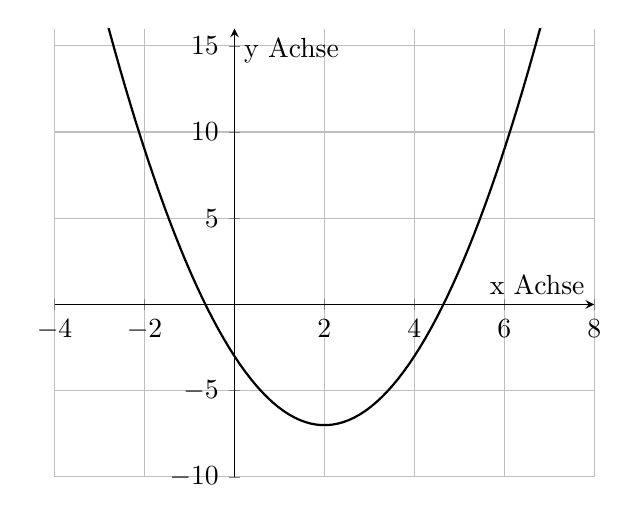
\begin{tikzpicture}
    \begin{axis}[
        axis x line=center,
        axis y line=center,
        domain=-4:8,
        grid=major,
        samples=100,
        xlabel={x Achse},
        xmax=8,
        xmin=-4,
        ylabel={y Achse},
        ymax=16,
        ymin=-10,
      ]
      \addplot[black, thick](x,x * x - 4 * x - 3);
    \end{axis}
  \end{tikzpicture}
  
  \[
    B = \interval[open]{-\infty}{1} \cup \interval[open]{3}{\infty}
  \]

%% c)
\item Stelle Sie $C = \{ x \in \mathbb{R} | \frac{2x + 1}{x - 1} \leq x - 1 \}$ als Intervall dar.
  \begin{align*}
    \frac{2x + 1}{x - 1} &\leq x - 1        &&| * (x - 1), \text{ $x$ ist für $1$ nicht definiert} \\
                  2x + 1 &\leq (x - 1)^2 \\
                  2x + 1 &\leq x^2 - 2x + 1 &&| -(2x + 1)\\
                       0 &\leq x^2 - 4x \\
  \end{align*}
  \begin{align*}
    x_{1|2} &= -\frac{(-4)}{2} \pm \sqrt{\frac{4^2}{4} - 0} \\
            &= 2 \pm \sqrt{4} \\
            &= 2 \pm 2 \\
  \end{align*}
  \[
    x_1 = 0, x_2 = 4
  \]

  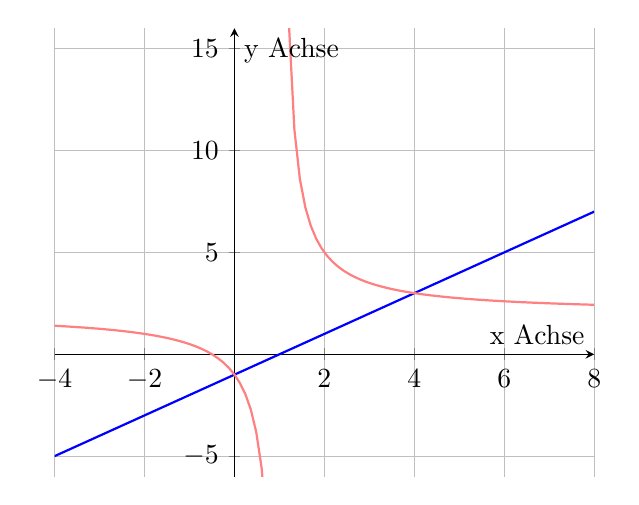
\begin{tikzpicture}
    \begin{axis}[
        axis x line=center,
        axis y line=center,
        domain=-4:8,
        grid=major,
        restrict y to domain=-10:20,
        samples=100,
        xlabel={x Achse},
        xmax=8,
        xmin=-4,
        ylabel={y Achse},
        ymax=16,
        ymin=-6,
      ]
      \addplot[blue, thick] { x - 1 };
      \addplot[red!50, thick] {(2*x + 1) / (x - 1) };
    \end{axis}
  \end{tikzpicture}
  \[
    C = \interval[open right]{0}{1} \cup \interval[open right]{4}{+\infty}
  \]

%% d)
\item
  \begin{align*}
    A \cup B        &= \interval[open left]{2}{4} \cup \interval[open]{3}{+\infty} \cup \interval[open]{-\infty}{1} \\
                    &= \interval[open]{-\infty}{1} \cup \interval[open]{2}{\infty} \\
    A \cap C        &= \{ 4 \} \\
    A \cup B \cup C &= \interval[open]{-\infty}{1} \cup \interval[open]{2}{\infty} \\
    A \cap B \cap C &= \{ 4 \} \\
  \end{align*}
\end{enumerate}

\section*{Hausaufgabe 3}

\begin{enumerate}[a)]
%% a)
\item $A \coloneqq \{ \frac{x}{x + 1} | x \in \mathbb{R}, x > -1 \}$
  \begin{align*}
    \text{inf}(A) &= -1 \\
    \text{sup}(A) &= 1 \\
  \end{align*}
  \begin{itemize}
  \item $A$ hat kein Minimum, da das Infimum von $A$ nicht in der Menge liegt 
  \item $A$ hat kein Minimum, da das Supremum von $A$ nicht in der Menge liegt 
  \end{itemize}
%% b)
\item $B \coloneqq \{ 1 + 2 * (-1)^n + 3 * (-1)^{\frac{n*(n - 1)}{2}} | n \in \mathbb{N}\}$

  \[
    B \coloneqq \{ 2, 0, -4, 6 \} 
  \]
  \begin{itemize}
  \item es existiert ein Minimum, da $\text{inf}(B) = -4$ in der Menge liegt 
  \item es existiert ein Minimum, da $\text{sup}(B) = 6$ in der Menge liegt 
  \end{itemize}

\end{enumerate}
\end{document}